\documentclass[dvipsnames,tikz]{standalone}
\usepackage{amsmath}
\usepackage{xcolor}
\usepackage{tikz}
\usetikzlibrary{calc}
\usetikzlibrary{decorations.pathreplacing,calligraphy,3d}


\begin{document}
	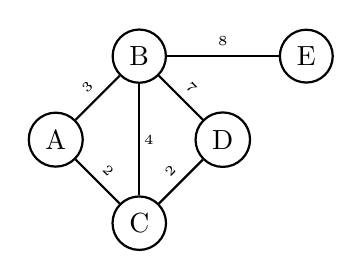
\begin{tikzpicture}[node distance={15mm}, thick, main/.style = {draw, circle}] 
		\node[main] (A) {A}; 
		\node[main] (B) [above right of=A] {B};
		\node[main] (C) [below right of=A] {C}; 
		\node[main] (D) [above right of=C] {D};
		\node[main] (E) [above right of=D] {E}; 
		
		\begin{scope}[font=\tiny]
			\draw (C) -- node[midway, above, sloped] {2} (A);
			\draw (A) -- node[midway, above, sloped] {3} (B);
			\draw (B) -- node[midway, right, xshift=-2pt] {4} (C);
			\draw (D) -- node[midway, above, sloped] {7} (B);
			\draw (B) -- node[midway, above, sloped] {8} (E);
			\draw (C) -- node[midway, above, sloped] {2} (D);
		\end{scope}
	\end{tikzpicture} 
	
\end{document}